\documentclass[12pt]{article}

\usepackage[margin=0.7in]{geometry}
\usepackage{amsfonts, amssymb, amsmath}
\usepackage[none]{hyphenat}
\usepackage{fancyhdr}
\usepackage{float}
\usepackage{setspace}
\usepackage{graphicx}
\usepackage{hyperref}
\usepackage[table]{xcolor}
\usepackage{multirow}
\usepackage{color}
\usepackage{listings}
\usepackage{enumitem}

\pagestyle{fancy}
\fancyhead{}
\fancyfoot{}
\fancyhead[L]{\MakeUppercase{PH1202 Expt. No.: 01}}
\fancyhead[R]{\slshape Priyanshu Mahato: \href{mailto:pm21ms002@iiserkol.ac.in}{\color{purple}pm21ms002@iiserkol.ac.in}}
\fancyfoot[C]{\thepage}

\renewcommand{\footrulewidth}{1pt}
% \renewcommand{\baselinestretch}{1.2}
\renewcommand\thesection{\arabic{section}}

\setlength{\headheight}{16pt}
\setlength{\parindent}{0em}
\setlength{\parskip}{1.5em}

\lstset{frame=tb,
	language=Python,
	aboveskip=3mm,
	belowskip=3mm,
	showstringspaces=false,
	columns=flexible,
	basicstyle={\small\ttfamily},
	numbers=none,
	numberstyle=\tiny\color{gray},
	keywordstyle=\color{blue},
	commentstyle=\color{dkgreen},
	stringstyle=\color{mauve},
	breaklines=true,
	breakatwhitespace=true,
	tabsize=3
}

\definecolor{dkgreen}{rgb}{0,0.6,0}
\definecolor{gray}{rgb}{0.5,0.5,0.5}
\definecolor{mauve}{rgb}{0.58,0,0.82}
\definecolor{ChadDarkBlue}{rgb}{.1,0,.2}  
\definecolor{ChadBlue}{rgb}{.1,.1,.5}  
\definecolor{ChadRoyal}{rgb}{.2,.2,.8}  
%\definecolor{ChadGreen}{rgb}{0,.35,.1}
%\definecolor{ChadGreen}{rgb}{0,.5,.25}  % Too bright
%\definecolor{ChadGreen}{rgb}{0,.4,.2}    % Still too bright
\definecolor{ChadGreen}{rgb}{0.5, 0, 0.2}    % Dark Green
%\definecolor{ChadRed}{rgb}{.8,.1,.2}    % Too bright
\definecolor{ChadRed}{rgb}{.5,0,.5}  % purple

\begin{document}
	\thispagestyle{empty}
	\begin{titlepage}
		\begin{center}
			\vspace{2cm}
			\huge\textbf{PH1202}\\
			\vspace{1cm}
			\large\textbf{Physics Laboratory II}
			\vfill
			\line(1, 0){470}\\[14pt]
			\huge\textbf{\color{ChadBlue}\sffamily Experiment Number - 1}\\[10pt]
			\Large\textbf{\color{mauve}\sffamily Determination of the acceleration due to gravity}\\[14pt]
			\line(1, 0){470}
			\vfill
			By: Priyanshu Mahato (\href{mailto:pm21ms002@iiserkol.ac.in}{\emph{\color{dkgreen}pm21ms002@iiserkol.ac.in}})\\
			Roll No.: pm21ms002\\
			\today
		\end{center}
	\end{titlepage}

	\section{Aim}
	In this project, we will have to determine the value of the acceleration due to gravity at our place (wherever we are) by measuring the time period of a simple pendulum. 
	
	\section{Equipments}
	The experiment required the use of the following equipments
	\begin{enumerate}
		\item Inextensible String
		\item Bob (here, Ball)
		\item Rigid Support
		\item Stopwatch/Timer
	\end{enumerate}

	\section{Description and Image of the Setup}
	\begin{figure}[H]
		\centering
		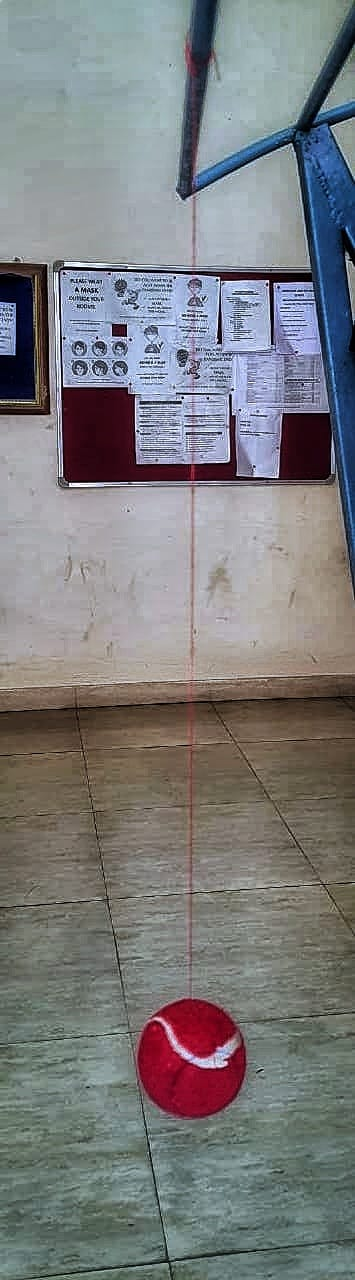
\includegraphics[scale=0.2]{Experiment}
		\caption{Image of the Setup}
	\end{figure}

	
	First a thread was hung from a rigid support (here, cloth hanger). Then, a ball was tied to the free end of the string as a bob. Then, we measure the time taken for 20 oscillations (5 to 6 readings) by taking different lengths of the string. After that we try to calculate the value of \emph{g} (acceleration due to gravity) using the formula: $$T = 2\pi \sqrt{\frac{l}{g}}$$The readings were as follows:
	
	\section{Readings/Tables}
	
	For string length 55.75 \emph{cm}:-
	
	\begin{table}[H]
		\begin{tabular}{|l|l|l|l|l|}
			\hline
			Sl. No. & Oscillations & Total Time Taken & Time per Oscillation (sec) & Average                \\ \hline
			1       & 20           & 30.26            & 1.513                      & \multirow{12}{*}{1.53} \\ \cline{1-4}
			2       & 20           & 29.50            & 1.475                      &                        \\ \cline{1-4}
			3       & 20           & 30.89            & 1.5445                     &                        \\ \cline{1-4}
			4       & 20           & 30.76            & 1.538                      &                        \\ \cline{1-4}
			5       & 20           & 30.55            & 1.5275                     &                        \\ \cline{1-4}
			6       & 20           & 30.72            & 1.536                      &                        \\ \cline{1-4}
			7       & 20           & 31.20            & 1.56                       &                        \\ \cline{1-4}
			8       & 20           & 30.9             & 1.545                      &                        \\ \cline{1-4}
			9       & 20           & 30.19            & 1.5095                     &                        \\ \cline{1-4}
			10      & 20           & 30.75            & 1.5375                     &                        \\ \cline{1-4}
			11      & 20           & 30.35            & 1.5175                     &                        \\ \cline{1-4}
			12      & 20           & 30.99            & 1.5495                     &                        \\ \hline
		\end{tabular}
	\end{table}

	For string length 71.25 \emph{cm}:-

	\begin{table}[H]
		\begin{tabular}{|l|l|l|l|l|}
			\hline
			Sl. No. & Oscillations & Total Time Taken & Time per Oscillation (sec) & Average               \\ \hline
			1       & 20           & 34.41            & 1.72                       & \multirow{7}{*}{1.71} \\ \cline{1-4}
			2       & 20           & 34.37            & 1.72                       &                       \\ \cline{1-4}
			3       & 20           & 34.40            & 1.72                       &                       \\ \cline{1-4}
			4       & 20           & 34.37            & 1.72                       &                       \\ \cline{1-4}
			5       & 20           & 34.21            & 1.71                       &                       \\ \cline{1-4}
			6       & 20           & 34.12            & 1.71                       &                       \\ \cline{1-4}
			7       & 20           & 34.17            & 1.71                       &                       \\ \hline
		\end{tabular}
	\end{table}

	\pagebreak

	For string length 96.05 \emph{cm}:-

	\begin{table}[H]
		\begin{tabular}{|l|l|l|l|l|}
			\hline
			Sl. No. & Oscillations & Total Time Taken & Time per Oscillation (sec) & Average               \\ \hline
			1       & 20           & 39.72            & 1.99                       & \multirow{6}{*}{1.99} \\ \cline{1-4}
			2       & 20           & 39.70            & 1.99                       &                       \\ \cline{1-4}
			3       & 20           & 39.71            & 1.99                       &                       \\ \cline{1-4}
			4       & 20           & 39.69            & 1.98                       &                       \\ \cline{1-4}
			5       & 20           & 39.72            & 1.99                       &                       \\ \cline{1-4}
			6       & 20           & 39.74            & 1.99                       &                       \\ \hline
		\end{tabular}
	\end{table}

	For string length 120.00 \emph{cm}:-
	
	\begin{table}[H]
		\begin{tabular}{|l|l|l|l|l|}
			\hline
			Sl. No. & Oscillations & Total Time Taken & Time per Oscillation (s) & Average              \\ \hline
			1       & 20           & 44.61      & 2.23                     & \multirow{5}{*}{2.22} \\ \cline{1-4}
			2       & 20           & 44.81      & 2.24                     &                       \\ \cline{1-4}
			3       & 20           & 44.20      & 2.21                     &                       \\ \cline{1-4}
			4       & 20           & 44.43      & 2.22                     &                       \\ \cline{1-4}
			5       & 20           & 44.09      & 2.20                     &                       \\ \hline
		\end{tabular}
	\end{table}

	For string length 139.75 \emph{cm}:-

	\begin{table}[H]
		\begin{tabular}{|l|l|l|l|l|}
			\hline
			Sl. No. & Oscillations & Total Time Taken & Time per Oscillation (sec) & Average                \\ \hline
			1       & 20           & 47.87            & 2.39                       & \multirow{10}{*}{2.38} \\ \cline{1-4}
			2       & 20           & 47.57            & 2.38                       &                        \\ \cline{1-4}
			3       & 20           & 47.67            & 2.38                       &                        \\ \cline{1-4}
			4       & 20           & 47.49            & 2.37                       &                        \\ \cline{1-4}
			5       & 20           & 47.44            & 2.37                       &                        \\ \cline{1-4}
			6       & 20           & 47.32            & 2.37                       &                        \\ \cline{1-4}
			7       & 20           & 47.42            & 2.37                       &                        \\ \cline{1-4}
			8       & 20           & 47.52            & 2.38                       &                        \\ \cline{1-4}
			9       & 20           & 47.34            & 2.37                       &                        \\ \cline{1-4}
			10      & 20           & 47.47            & 2.37                       &                        \\ \hline
		\end{tabular}
	\end{table}

	\section{Calculations and Results}
	
	\begin{figure}[H]
		\centering
		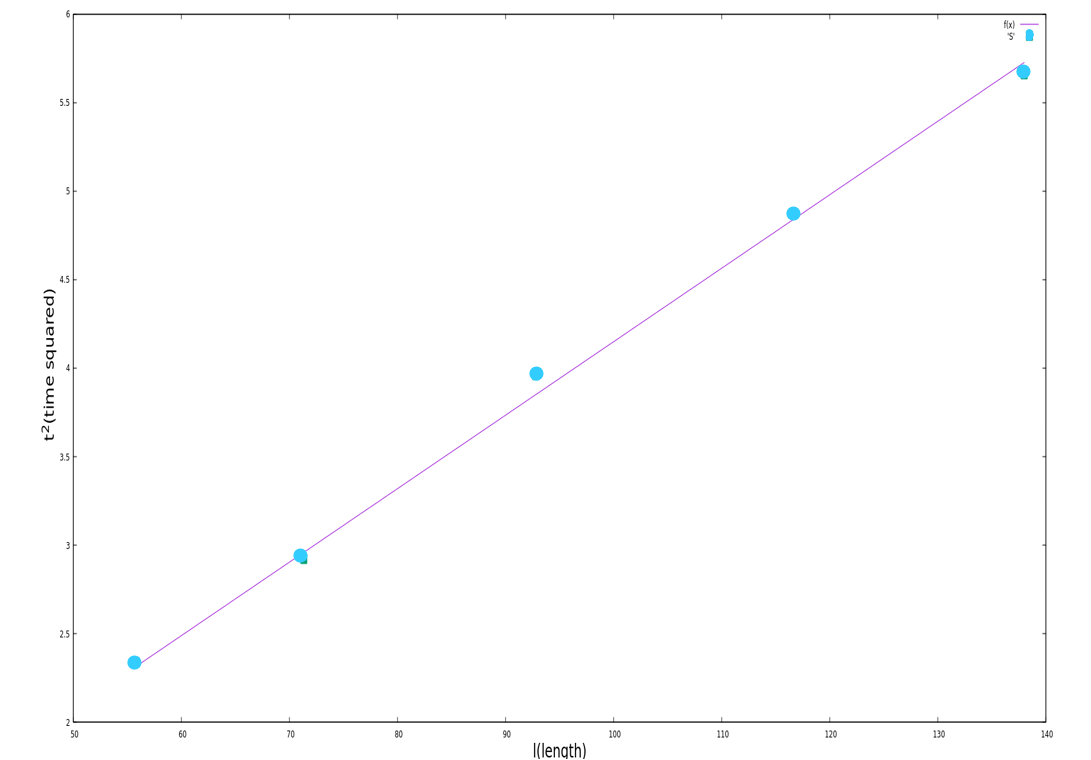
\includegraphics[scale=0.7]{photo}
		\caption{Graph of $t^{2}$ vs. $l$}
	\end{figure}

	From the formula $T = 2\pi \sqrt{\frac{l}{g}}$, we get, $$T^{2} = 4\pi^{2} \frac{l}{g}$$
	$$\Rightarrow g = 4\pi^{2} \frac{l}{T^{2}}$$
	$$Slope = \frac{T^{2}}{l} = \frac{4\pi^{2}}{g} = 0.041038\ cm^{-1} s^{2}\ (from\ graph)$$
	$$\Rightarrow \frac{4\pi^{2}}{g} = 0.041038\ cm^{-1} s^{2}$$
	$$\Rightarrow g = \frac{4\pi^{2}}{ 0.041038}\ cms^{-2} = 961.997\ cms^{-2} \approxeq 9.62\ ms^{-2}$$
	$$\boxed{g \approxeq 9.62\ ms^{-2}}$$
	
	\section{Error Analysis}
	
	The true/literature value of acceleration due to gravity is taken as \textbf{9.8 \emph{$ms^{-2}$}}. 
	
	\begin{align*} 
	Absolute\ Error &= |\texttt{True\ Value - Calculated\ Value}|\\
	&= |9.8 - 9.62|\\
	&= 0.18\ ms^{-2}
	\end{align*}

	\begin{align*}
		Percentage\ Error &= \frac{Absolute\ Error}{True\ Value} \times 100\%\\
		&= \frac{0.18}{9.8} \times 100\% \\
		&\approx 1.84\%
	\end{align*}

	\section{Systemic Error Analysis}
	
	From the equation, $$g = \frac{4\pi^{2}l}{T^{2}}$$
	
	Since we are using Physical Instruments to measure the parameters $l$ and $T$, we are bound to have error/uncertainty in our calculated value of $g$. Using Partial Derivatives in the above equation, we get, $$\frac{\delta(g)}{g} = \left|\frac{1}{l}\right|\delta l + \left|\frac{2}{T}\right|\delta T$$
	
	\pagebreak
	
	Now, substituting different parameters and least counts of instruments as individual errors in the equation, we obtain:-
	
	\begin{enumerate}
		\item For $l = 139.75\ cm$ $$\frac{\delta g}{g} = 0.9\%$$
		\item For $l = 120.00\ cm$ $$\frac{\delta g}{g} = 0.98\%$$
		\item For $l = 96.05\ cm$ $$\frac{\delta g}{g} = 1.1\%$$
		\item For $l = 71.25\ cm$ $$\frac{\delta g}{g} = 1.3\%$$
		\item For $l = 55.75\ cm$ $$\frac{\delta g}{g} = 1.5\%$$
	\end{enumerate}

	\section{Discussion}
	
	The nature of the plot is a straight line which is also true as per the equation, $$T = 2\pi \sqrt{\frac{l}{g}}$$
	
	To reduce the error we have allowed the ball to oscillate for some time to reduce the effect of torsion. We will also need to consider the motion to be planar. We also need to make sure that the oscillations need to be performed with the string at a very small angle from the equilibrium position. Otherwise, the above formula will not hold. 
	
	\section{Sources of Error}
	
	\begin{enumerate}[label=\alph*]
		\item There might be slight torsion in the string used.
		\item The string might be slightly extensible.
		\item Ball might not have uniform mass distribution and may not be perfectly spherical.
		\item Air resistance might come into play, but here it is neglected.
		\item Human sources of Error like stopping the stopwatch at exactly 20 oscillations of the pendulum, etc.
	\end{enumerate}
	
\end{document}